\chapter{Materiales y M├®todos}
\label{chap:materiales_metodos}

\noindent Este cap├¡tulo detalla la metodolog├¡a empleada en la investigaci├│n, incluyendo el dise├▒o del estudio, la caracterizaci├│n de la poblaci├│n participante, la definici├│n operacional de variables, los instrumentos de recolecci├│n de datos biom├®tricos y el protocolo de an├ílisis estad├¡stico implementado. Describimos el procedimiento completo desde la selecci├│n del Apple Watch como dispositivo wearable bajo los paradigmas de vida libre y \textit{Bring Your Own Device} (BYOD), seguido del protocolo de extracci├│n de datos mediante el ecosistema HealthKit, hasta la validaci├│n del sistema de inferencia difusa con estrategia Leave-One-User-Out, lo cual garantiza la reproducibilidad y transparencia metodol├│gica necesarias para la replicaci├│n de los hallazgos en estudios futuros.

% ============================================================================
\section{Dise├▒o del Estudio}
\label{sec:diseno}
% ============================================================================

Empleamos un dise├▒o cuantitativo, observacional, longitudinal retrospectivo con seguimiento multianual (2021-2024) de una cohorte de 10 participantes adultos. El dise├▒o se bas├│ en la validaci├│n convergente de un sistema de inferencia difusa tipo Mamdani contra una clasificaci├│n de referencia emp├¡rica (verdad operativa, GO) derivada de un an├ílisis de conglomerados no supervisado sobre datos biom├®tricos semanales agregados.

La unidad de an├ílisis correspondi├│ a semanas completas de monitoreo generadas a partir de los 9,185 d├¡as v├ílidos recopilados (1,385 semanas totales), de las cuales 1,337 cumplieron los criterios de calidad (ÔëÑ3 d├¡as con datos y Ôëñ60\% de imputaci├│n). Cada observaci├│n semanal integr├│ la mediana (p50) y el rango intercuart├¡lico (IQR) de cuatro variables biom├®tricas derivadas: Actividad Relativa, Super├ívit Cal├│rico Basal, Variabilidad de Frecuencia Card├¡aca (HRV-SDNN) y Delta Card├¡aco.

\subsection{Pivote Metodol├│gico}
\label{subsec:pivote_metodologico}

El planteamiento inicial del proyecto fue correlacional: busc├íbamos predecir el puntaje del cuestionario SF-36 (aplicado una sola vez por participante) a partir de las series biom├®tricas capturadas por el Apple Watch. Durante la fase piloto validamos que esta estrategia no era viable y adoptamos un enfoque metodol├│gico diferente, centrado en la convergencia entre patrones objetivos (clustering K-Means) y un sistema difuso basado en conocimiento experto. Fundamentamos este pivote en tres razones convergentes documentadas en la literatura:

\begin{enumerate}
    \item \textbf{Limitaciones de potencia estad├¡stica:} Con N=10 participantes, el poder para detectar correlaciones moderadas (r<0.70) entre variables biom├®tricas y SF-36 es insuficiente (1-$\beta$<0.50). Healy et al. \cite{Healy2024} reportan hallazgos convergentes: correlaciones d├®biles-moderadas (r=0.3-0.5, no significativas) entre cuestionarios de actividad f├¡sica y m├®tricas objetivas de wearables en cohortes N<15.
    
    \item \textbf{Baja adherencia al cuestionario:} Solo 8 de 10 participantes completaron el SF-36, y el análisis retrospectivo reveló correlaciones mayormente no significativas (p>0.05) excepto para Salud Mental (ver Sección \ref{subsec:sf36_exploratorio}).
    
    \item \textbf{Autopercepci├│n vs. comportamiento objetivo:} Prince et al. \cite{Prince2008} demuestran que autorreportes y mediciones objetivas representan constructos relacionados pero no intercambiables, con concordancia limitada (Kappa<0.50) debido a sesgos de deseabilidad social y error de memoria.
\end{enumerate}

En su lugar, adoptamos una estrategia de validación interna basada en la convergencia entre dos paradigmas: uno empírico (descubrimiento de patrones mediante agrupamiento K-Means) y uno experto (modelado basado en conocimiento mediante lógica difusa Mamdani). Este enfoque, validado por \cite{Goncalves2021} en clasificación de estabilidad humana, permite aprovechar la riqueza del conjunto de datos longitudinal (n=1,337 semanas) en lugar de limitarse a comparaciones inter-usuario con potencia estadística reducida.

% ============================================================================
\section{T├®cnicas y Procedimiento}
\label{sec:tecnicas_procedimiento}
% ============================================================================

\subsection{Selecci├│n del Dispositivo}
\label{subsec:seleccion_dispositivo}

Para la selecci├│n del dispositivo de monitoreo, utilizamos una base de datos detallada que analiza 423 dispositivos de 133 marcas, divididos en 187 monitores de actividad f├¡sica y 236 relojes inteligentes lanzados desde 2011 \citep{Henriksen2021ReplicationData}. Esta base permiti├│ identificar las capacidades t├®cnicas de cada dispositivo, como sensores incluidos y su utilidad en la medici├│n de patrones de actividad f├¡sica (AF) y comportamiento sedentario (CS).

\subsection{Análisis de Sensores}
\label{subsec:analisis_sensores}

Del análisis de los 423 dispositivos, observamos que todos cuentan con un acelerómetro, esencial para medir la intensidad y frecuencia del movimiento y facilitar así la evaluación de la AF \citep{Henriksen2021ReplicationData}. Sin embargo, solo el 38.3\% de los dispositivos (162 de 423) incluyen un sensor de fotopletismografía (PPG), crucial para medir frecuencia y variabilidad cardíaca, indicadores relevantes para evaluar esfuerzo físico y salud cardiovascular \citep{Pinto2023Physiology}. Aunque en 2011 solo el 14\% de los wearables incluían PPG, esta tecnología creció significativamente y alcanzó un 55\% en los dispositivos lanzados en 2016, lo cual refleja su creciente relevancia en la monitorización de la salud \citep{Henriksen2018}.

Otros sensores, como el giroscopio (23.9\%) y el GPS (29.6\%), tambi├®n destacan por su utilidad. El giroscopio mejora la detecci├│n de posturas y rotaciones corporales, mientras que el GPS permite registrar trayectorias, ├║til en actividades al aire libre. Sensores menos comunes, como el magnet├│metro (18.2\%) y el bar├│metro (13.5\%), tienen aplicaciones espec├¡ficas, pero son menos relevantes para este estudio \citep{Henriksen2018}.

\subsection{Elecci├│n del Apple Watch}
\label{subsec:eleccion_apple_watch}

El an├ílisis de mercado identific├│ a Apple como el l├¡der en la categor├¡a de relojes inteligentes, con un 49\% de la cuota global, seguido por Samsung (15\%) y Garmin (11\%) \citep{Canalys2024Wearables}. Esta predominancia y la uniformidad en sus dispositivos justifican la elecci├│n del Apple Watch como el dispositivo m├ís adecuado, asegurando una mayor representatividad de datos y compatibilidad con herramientas de an├ílisis avanzadas. La \Cref{tab:wearables_comparison_extended} resume la matriz de decisi├│n empleada, incorporando a los principales proveedores disponibles en M├®xico.

\begin{table}[H]
    \centering
    \caption{Matriz de decisi├│n extendida para selecci├│n de dispositivo wearable}
    \label{tab:wearables_comparison_extended}
    \begingroup
    \setlength{\tabcolsep}{4pt}
    \renewcommand{\arraystretch}{1.15}
    \footnotesize
    \begin{tabularx}{\textwidth}{@{}p{3.0cm}*{5}{>{\raggedright\arraybackslash}X}@{}}
        \toprule
        \textbf{Criterio} & \textbf{Apple Watch} & \textbf{Fitbit} & \textbf{Garmin} & \textbf{Polar} & \textbf{Huawei} \\
        \midrule
        Penetraci├│n en M├®xico & Alta & Media & Media-baja & Baja & Media \\
        Sensores validados & Sí (todos) & Sí (núcleo) & Sí (núcleo) & Sí (núcleo) & Parcial \\
        Exportaci├│n de datos & HealthKit (XML/API) & Fitbit Web API & Garmin Health API & Polar AccessLink & Huawei Health API (limitada) \\
        Consistencia HW/SW & Alta (ecosistema cerrado) & Media & Alta & Media & Baja (fragmentaci├│n) \\
        SDK / Documentación & HealthKit (extensa) & API con foros activos & Documentación integral & Moderada (deportiva) & Limitada/básica \\
        \bottomrule
    \end{tabularx}
    \endgroup
\end{table}

\FloatBarrier

\subsection{Protocolo del Instrumento}
\label{subsec:protocolo_instrumento}

Para la implementaci├│n del instrumento se estableci├│ un protocolo espec├¡fico para la extracci├│n y procesamiento de variables biom├®tricas obtenidas de dispositivos Apple Watch, utilizando los archivos exportados por la aplicaci├│n Apple Health. Este enfoque permiti├│ recopilar las m├®tricas necesarias sin desarrollar una aplicaci├│n personalizada ni programar en Swift, lo cual garantiz├│ la integridad y seguridad de los datos a trav├®s de un procedimiento manual estructurado y replicable \citep{Apple2024HealthKit}.



La \Cref{fig:diagrama_flujo} ilustra la secuencia completa del proceso metodol├│gico, desde la recepci├│n de archivos \path{export.zip} generados por Apple Health hasta la consolidaci├│n de variables semanales para el an├ílisis estad├¡stico. El proceso se estructur├│ en cinco etapas: (1) recepci├│n y almacenamiento seguro, (2) descompresi├│n y conversi├│n XMLÔåÆCSV, (3) extracci├│n de m├®tricas espec├¡ficas con filtrado por \texttt{sourceName}, (4) manejo de datos faltantes y valores at├¡picos, y (5) consolidaci├│n en un DataFrame con etiquetas estandarizadas.

\begin{figure}[H]
    \centering
    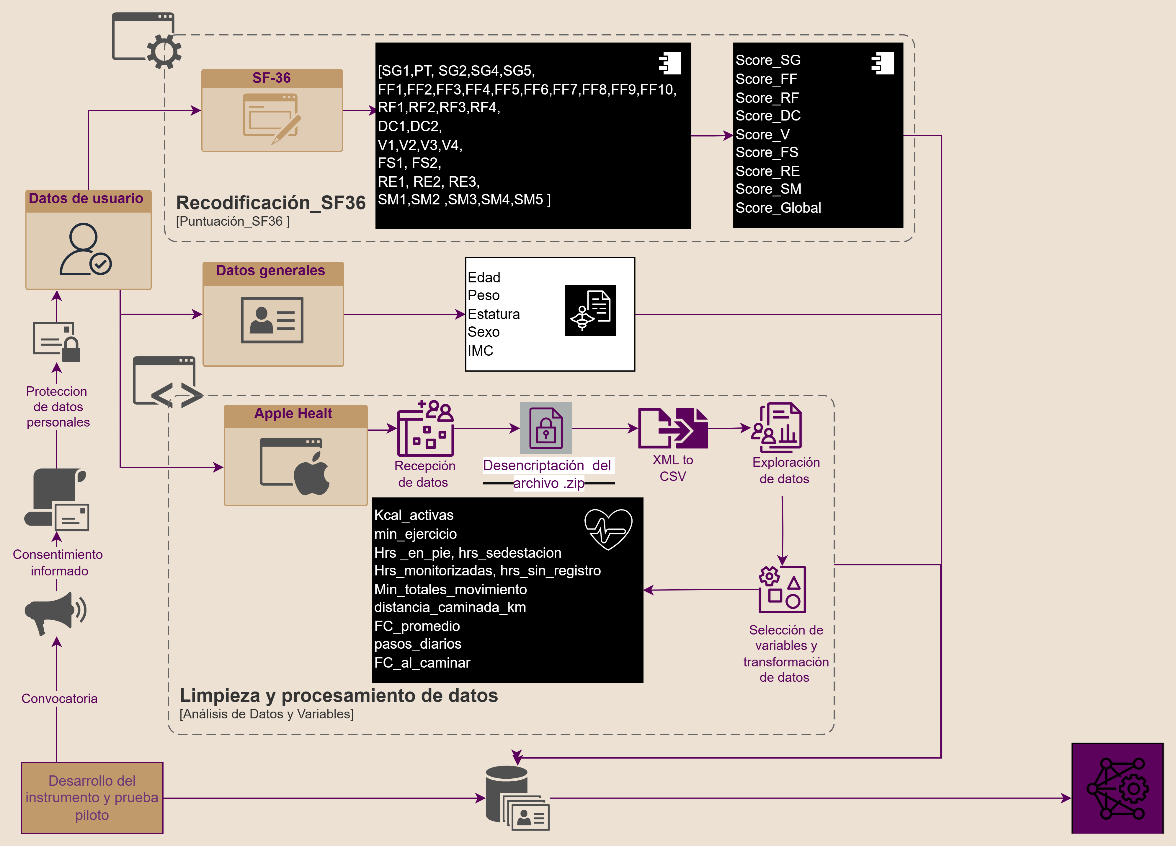
\includegraphics[width=0.9\textwidth]{figuras/diagrama_de_flujo_fig3.png}
    \caption{Diagrama de flujo del proceso metodol├│gico completo}
    \label{fig:diagrama_flujo}
\end{figure}

Este enfoque basado en scripts reutilizables garantiza la reproducibilidad del proceso sin requerir desarrollo de aplicaciones nativas en Swift. Los participantes generaron un archivo \path{export.zip} a trav├®s de la aplicaci├│n Apple Health en sus dispositivos. Recibimos y almacenamos cada archivo en un entorno seguro, asign├índole un c├│digo ├║nico de participante para asegurar la confidencialidad y trazabilidad de la informaci├│n. Posteriormente descomprimimos los archivos para acceder a los datos en formato XML. Utilizamos el script de c├│digo abierto \nolinkurl{apple_health_data_converter.py}, disponible en GitHub, para convertir los archivos XML a formato CSV, facilitando su manejo y an├ílisis estad├¡stico posterior \citep{Gaur2024AppleHealth}.

Identificamos los archivos \nolinkurl{ActiveEnergyBurned.csv}, \nolinkurl{AppleExerciseTime.csv}, \nolinkurl{AppleStandHour.csv}, \nolinkurl{AppleStandTime.csv}, \nolinkurl{DistanceWalkingRunning.csv}, \nolinkurl{HeartRate.csv}, \nolinkurl{StepCount.csv}, \nolinkurl{WalkingHeartRateAverage.csv} y extrajimos las m├®tricas espec├¡ficas relevantes para el estudio \citep{Apple2024HealthKit,Gaur2024AppleHealth}. Posteriormente desarrollamos un c├│digo personalizado en Python utilizando las bibliotecas \texttt{pytz} para el manejo de zonas horarias, \texttt{pandas} para la manipulaci├│n de datos y \texttt{numpy} para operaciones num├®ricas. Este c├│digo convirti├│ las fechas y horas de cada registro al formato est├índar y las ajust├│ al huso horario correspondiente. Para garantizar que los datos provinieran exclusivamente del Apple Watch de cada participante, filtramos los registros utilizando la columna \texttt{sourceName}, seleccionando ├║nicamente los datos asociados al dispositivo espec├¡fico del participante y excluyendo posibles registros de otros dispositivos o aplicaciones vinculadas.

\begin{figure}[htbp]
    \centering
    \caption{Algoritmo 1. Preprocesamiento XML $\rightarrow$ CSV diario}
    \label{alg:xml_csv}
    \begin{minipage}{0.95\textwidth}
        \textbf{Entrada:} archivo \path{export.zip} por participante \\
        \textbf{Salida:} \path|DB_u{id}.csv| con columnas [fecha, pasos, calorías, FC\_reposo, HRV\_SDNN, \ldots]\\[4pt]
        \begin{enumerate}[label=\textbf{Paso \arabic*:}, leftmargin=*]
            \item Analizar el archivo XML: \texttt{tree = parse(xml\_file)}.
            \item Extraer los nodos \texttt{Record}: \texttt{records = tree.findall("Record")}.
            \item Inicializar un \texttt{DataFrame} vacío donde se almacenarán los registros consolidados.
            \item Recorrer cada \texttt{record} y filtrar ├║nicamente los que provienen del Apple Watch (\texttt{sourceName} contiene ``Apple Watch''); guardar \texttt{type}, \texttt{value} y la fecha (\texttt{startDate}).
            \item Agrupar los registros por fecha mediante un pivote que transforma las filas en columnas por tipo de m├®trica.
            \item Exportar el \texttt{DataFrame} resultante a CSV con la nomenclatura \texttt{DB\_u\{id\}.csv}.
        \end{enumerate}
    \end{minipage}
\end{figure}
Para el manejo de datos identificamos registros con valores faltantes, nulos o atípicos. Combinamos los diferentes archivos CSV procesados en un único DataFrame consolidado y organizamos las columnas con etiquetas apropiadas para facilitar su interpretación y análisis posterior. Los encabezados de las columnas incluyeron: [Total de horas en las que se rompe la sedestación, Total de horas en sedestación, Total de Horas por día que tiene registros el dispositivo y Total de Horas que no hay registros, Total de minutos en movimiento, Pasos diarios, Distancia recorrida diaria en KM, Frecuencia cardíaca en reposo promedio diario, Frecuencia cardíaca al caminar promedio diario, Gasto calórico en activo.]

% ============================================================================
\section{Poblaci├│n de Estudio}
\label{sec:poblacion_estudio}
% ============================================================================

La cohorte final del estudio estuvo compuesta por 10 adultos j├│venes (5 mujeres, 5 hombres; rango etario: 25-39 a├▒os) reclutados mediante convocatoria abierta en la Facultad de Medicina y Ciencias Biom├®dicas de la Universidad Aut├│noma de Chihuahua entre septiembre de 2021 y enero de 2022.

\subsection{Estrategia de Reclutamiento}
\label{subsec:reclutamiento}

Empleamos un muestreo no probabilístico por conveniencia basado en el paradigma \textit{Bring Your Own Device} (BYOD; \cite{Doherty2021}). Basamos los criterios de inclusión en:

\begin{enumerate}
    \item Propiedad de un Apple Watch Series 3 o superior
    \item Uso continuo del dispositivo por al menos 6 meses previos (para minimizar efectos de habituaci├│n)
    \item Edad entre 18 y 65 a├▒os
    \item Capacidad ambulatoria sin limitaciones severas
    \item Disponibilidad para exportar datos hist├│ricos del ecosistema HealthKit
\end{enumerate}

\subsection{Tamaño de Muestra y Justificación Estadística}
\label{subsec:justificacion_n}

Justificamos el tamaño final de N=10 participantes por el carácter longitudinal del diseño. Cada participante generó un promedio de 133.7 semanas válidas (mediana: 131 semanas; rango: 7-298 semanas), lo cual resultó en 1,337 observaciones semanales independientes para el modelado.

Este enfoque se alinea con el paradigma de \textbf{muestras densamente monitoreadas} (\textit{intensive longitudinal designs}; \cite{Bolger2013}), donde el poder estadístico proviene del número de observaciones temporales por sujeto (n$_{\text{obs}}$) más que del número de sujetos (N):

\begin{equation}
\text{Poder} \propto N \times \bar{n}_{\text{obs/sujeto}}
\label{eq:poder_longitudinal}
\end{equation}

Con N=10 y $\bar{n}_{\text{obs}}$=133.7, se obtuvo n$_{\text{total}}$=1,337, superando el mínimo recomendado (n$_{\text{total}} \geq$ 500) para agrupamiento estable y validación Leave-One-User-Out robusta \cite{Alinia2020}.

\subsection{Características Demográficas de la Cohorte}
\label{subsec:caracteristicas_cohorte}

La distribución balanceada por sexo (50\%/50\%) y el amplio rango de seguimiento (7-298 semanas; CV=86\%) permiten capturar heterogeneidad inter-sujeto e intra-sujeto, características esenciales para evaluar la robustez del sistema de inferencia difusa en condiciones de vida libre. Presentamos las características detalladas en la \Cref{tab:cohorte_caracteristicas}.

\begin{table}[htbp]
\centering
\caption{Características Demográficas de la Cohorte (N=10)}
\label{tab:cohorte_caracteristicas}
\begingroup
\setlength{\tabcolsep}{5pt}
\renewcommand{\arraystretch}{1.1}
\small
\begin{tabular}{@{}lccccc@{}}
\toprule
\textbf{Usuario} & \textbf{Sexo} & \textbf{Edad} & \textbf{IMC} & \textbf{Semanas} & \textbf{\% Válidas} \\
\midrule
u1 & F & 34 & 23.5 & 149 & 100\% \\
u2 & F & 37 & 26.6 & 7   & 100\% \\
u3 & F & 39 & 28.7 & 141 & 100\% \\
u4 & M & 25 & 30.9 & 14  & 100\% \\
u5 & F & 28 & 25.0 & 14  & 100\% \\
u6 & M & 34 & 30.9 & 278 & 100\% \\
u7 & M & 32 & 37.8 & 114 & 100\% \\
u8 & M & 29 & 28.1 & 191 & 100\% \\
u9 & M & 32 & 36.2 & 298 & 100\% \\
u10 & F & 28 & 21.6 & 131 & 100\% \\
\midrule
\textbf{Media┬▒SD} & 5M/5F & 31.8┬▒4.5 & 28.9┬▒5.1 & 133.7┬▒95.3 & 100\% \\
\bottomrule
\end{tabular}
\endgroup
\end{table}

\subsection{Análisis Descriptivo Previo a la Agregación}
\label{subsec:analisis_descriptivo}

Realizamos un an├ílisis descriptivo exhaustivo de los 9,185 d├¡as v├ílidos antes de derivar las variables semanales. La \Cref{tab:descriptivos_actualizados} resume los estad├¡sticos principales y evidencia coeficientes de variaci├│n superiores al 50\% en la mayor├¡a de las m├®tricas, lo cual anticipa la necesidad de estad├¡sticos robustos (medianas e IQR) y de un mecanismo de agregaci├│n temporal semanal.

\begin{table}[htbp]
    \centering
    \caption{Estadísticos descriptivos diarios (datos post-limpieza, $n=9{,}185$ días)}
    \label{tab:descriptivos_actualizados}
    \resizebox{\textwidth}{!}{%
    \begin{tabular}{@{}lrrrrrrrrrrrr@{}}
        \toprule
        \textbf{Variable} & \textbf{n} & \textbf{Media} & \textbf{DE} & \textbf{CV (\%)} & \textbf{Mediana} & \textbf{Q1} & \textbf{Q3} & \textbf{IQR} & \textbf{Mín} & \textbf{Máx} & \textbf{Test} & \textbf{$p$-valor} \\
        \midrule
        Pasos diarios & 9,185 & 6,001.6 & 3,283.6 & 54.7 & 5,489.0 & 3,779.0 & 7,657.0 & 3,878.0 & 11.5 & 25,511.7 & K-S & $< 0.001$ \\
        Calorías activas (kcal) & 9,185 & 595.9 & 450.7 & 75.6 & 517.7 & 322.1 & 767.4 & 445.3 & 0.1 & 18,313.1 & K-S & $< 0.001$ \\
        FC reposo (lpm) & 9,185 & 54.2 & 8.7 & 16.1 & 53.0 & 48.0 & 59.0 & 11.0 & 37.0 & 142.6 & K-S & $< 0.001$ \\
        FC al caminar (lpm) & 9,185 & 97.8 & 12.4 & 12.7 & 97.8 & 90.5 & 105.0 & 14.5 & 50.0 & 159.0 & K-S & $< 0.001$ \\
        HRV-SDNN (ms) & 9,185 & 49.4 & 17.2 & 34.8 & 48.4 & 36.2 & 60.4 & 24.2 & 9.8 & 135.4 & K-S & $< 0.001$ \\
        Horas monitoreadas & 9,185 & 15.4 & 5.2 & 33.8 & 15.0 & 13.0 & 18.0 & 5.0 & 1.0 & 65.0 & K-S & $< 0.001$ \\
        Actividad relativa & 9,185 & 0.14 & 0.10 & 73.2 & 0.13 & 0.08 & 0.18 & 0.09 & 0.00 & 2.15 & K-S & $< 0.001$ \\
        Superávit calórico (\%) & 9,185 & 32.6 & 23.0 & 70.6 & 28.0 & 19.9 & 40.9 & 21.0 & 0.0 & 817.1 & K-S & $< 0.001$ \\
        \bottomrule
    \end{tabular}}
\end{table}

Las distribuciones exhibieron colas pesadas hacia valores bajos de actividad (Figura~\ref{fig:histogramas_kde}), fen├│meno que explica por qu├® la partici├│n ├│ptima detectada por clustering fue $K=2$ (perfiles bajo y alto sedentarismo). Asimismo, los boxplots comparativos (Figura~\ref{fig:boxplots_comparativos}) muestran heterogeneidad inter-sujeto e intra-sujeto, reforzando la decisi├│n de utilizar mediana e IQR como descriptores semanales.

\begin{figure}[htbp]
    \centering
    
\includegraphics[width=0.9\textwidth]{figuras/histogramas_con_kde.png}
    \caption{Distribuciones diarias de variables clave con densidad KDE}
    \label{fig:histogramas_kde}
\end{figure}

\begin{figure}[htbp]
    \centering
    
\includegraphics[width=0.9\textwidth]{figuras/boxplots_comparativos.png}
    \caption{Boxplots comparativos que evidencian asimetría y outliers por usuario}
    \label{fig:boxplots_comparativos}
\end{figure}

Adicionalmente comparamos la variabilidad puramente observada con la variabilidad operativa posterior a la imputación jerárquica (Figura~\ref{fig:variabilidad_comparativa}). La imputación reduce la dispersión de biomarcadores como HRV-SDNN y la frecuencia cardíaca en reposo, pero mantiene la heterogeneidad legítima de los patrones de actividad. Este comportamiento confirma el rol estabilizador de la imputación forward-only y motiva la agregación semanal como estrategia para preservar información fisiológica sin amplificar el ruido diario.

\begin{figure}[htbp]
    \centering
    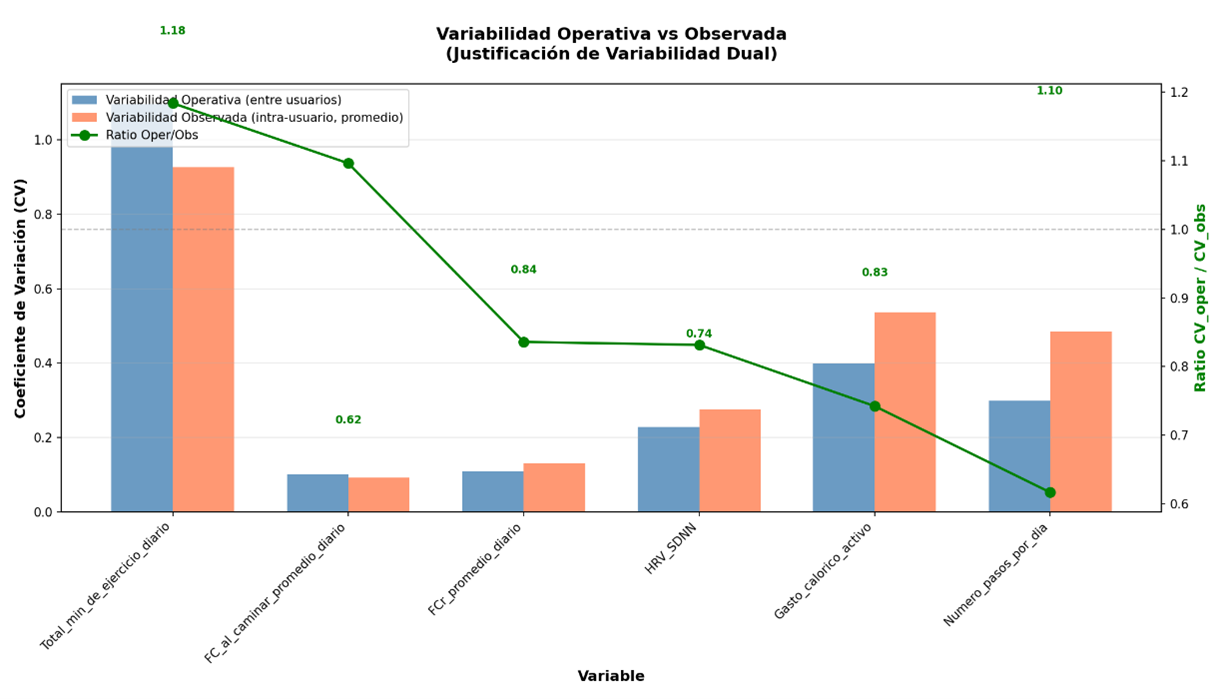
\includegraphics[width=0.95\textwidth]{figuras/variabilidadoperativa_vs_observada.png}
    \caption{Comparaci├│n de variabilidad observada vs.\ operativa despu├®s de imputaci├│n}
    \label{fig:variabilidad_comparativa}
\end{figure}

% ============================================================================
\section{Definici├│n Operacional de Variables}
\label{sec:definicion_operacional_variables}
% ============================================================================

\subsection{Relaci├│n entre Variables}
\label{subsec:relacion_variables}

El estudio eval├║a la convergencia entre dos representaciones del comportamiento sedentario semanal: (i) la verdad operativa obtenida mediante clustering K-Means sobre las variables biom├®tricas derivadas y (ii) la clasificaci├│n generada por el sistema de inferencia difusa Mamdani. Ambas se apoyan en las mismas entradas cuantitativas pero responden a paradigmas distintos (descubrimiento emp├¡rico vs.\ conocimiento experto), lo que permite medir la capacidad del modelo difuso para replicar patrones objetivos en condiciones de vida libre.

\subsection{Variables Independientes}
\label{subsec:variables_independientes}

Las variables independientes corresponden a las cuatro caracter├¡sticas biom├®tricas derivadas a nivel semanal, cada una representada por su mediana (p50) y rango intercuart├¡lico (IQR):
\begin{enumerate}[noitemsep]
    \item \textbf{Actividad relativa:} pasos normalizados por horas monitoreadas (kilopasos/hora).
    \item \textbf{Superávit calórico basal:} gasto calórico activo expresado como porcentaje de la TMB individual.
    \item \textbf{Delta cardíaco:} diferencia entre frecuencia cardíaca al caminar y en reposo.
    \item \textbf{HRV-SDNN:} variabilidad de la frecuencia cardíaca (desviación estándar de los intervalos NN).
\end{enumerate}
Estas ocho características (4 medianas + 4 IQR) alimentan tanto el algoritmo de clustering como el sistema de inferencia difusa.

\subsection{Variable Dependiente}
\label{subsec:variable_dependiente}

La variable dependiente corresponde a la clasificación semanal de sedentarismo. Para entrenar y evaluar el modelo difuso utilizamos la etiqueta binaria proveniente de la verdad operativa (clustering K-Means, $K=2$). El sistema Mamdani genera un índice continuo en $[0,1]$ que posteriormente se binariza mediante el umbral óptimo $\tau=0.30$, de forma que la comparación entre ambas representaciones cuantifica la concordancia empírico--experta.

\subsection{Variables de Control}
\label{subsec:variables_control}

Registramos edad, sexo, peso, estatura y versión del Apple Watch para monitorear posibles efectos confusores. Adicionalmente fijamos los hiperparámetros que afectan la reproducibilidad computacional (por ejemplo, \texttt{random\_state}=42 y \texttt{n\_init}=10 en K-Means) y documentamos el entorno de ejecución (scikit-learn 1.4, Python 3.11) para garantizar replicabilidad.

\subsection{Operacionalizaci├│n de las Variables}
\label{subsec:operacionalizacion_variables}

La estructura XML exportada por Apple HealthKit (\Cref{lst:xml_structure}) contiene la informaci├│n cruda que se transforma en el dataset diario consolidado. Cada nodo \texttt{Record} encapsula una m├®trica biom├®trica con su \texttt{type}, \texttt{value} y rango temporal.

\begin{figure}[htbp]
    \centering
    \begin{minipage}{0.9\textwidth}
\begin{verbatim}
<HealthData locale="es_MX">
  <Record type="HKQuantityTypeIdentifierStepCount"
          sourceName="Apple Watch de u1"
          sourceVersion="10.1.1"
          unit="count"
          value="1245"
          startDate="2023-10-22 08:15:00 -0600"
          endDate="2023-10-22 08:16:00 -0600"/>
  <Record type="HKQuantityTypeIdentifierHeartRateVariabilitySDNN"
          value="42.3"
          unit="ms"
          startDate="2023-10-22 23:59:59 -0600"
          endDate="2023-10-22 23:59:59 -0600"/>
  ...
</HealthData>
\end{verbatim}
    \end{minipage}
    \caption{Estructura XML de Apple Health Export (fragmento representativo)}
    \label{lst:xml_structure}
\end{figure}

A partir de esta base aplicamos el algoritmo de la Tabla~\ref{alg:xml_csv}, obteniendo un archivo \texttt{DB\_u\{id\}.csv} por participante que concentra las m├®tricas relevantes.

La calidad de los registros se evalu├│ mediante las m├®tricas de la Tabla~\ref{tab:data_quality_raw}. Estas cifras justifican tanto el filtro de 1,337 semanas v├ílidas (ver Secci├│n~\ref{sec:diseno}) como la posterior imputaci├│n jer├írquica para manejar los periodos donde la se├▒al fotopletismogr├ífica fue insuficiente.

\begin{table}[htbp]
    \centering
    \caption{M├®tricas de completitud por usuario (fase pre-imputaci├│n)}
    \label{tab:data_quality_raw}
    \small
    \begin{tabular}{@{}lrrrrr@{}}
        \toprule
        \textbf{Usuario} & \textbf{Días totales} & \textbf{Días válidos} & \textbf{Completitud (\%)} & \textbf{Missing FC (\%)} & \textbf{Missing HRV (\%)} \\
        \midrule
        u1 & 900 & 852 & 94.7 & 8.2 & 15.3 \\
        u2 & 850 & 801 & 94.2 & 9.1 & 17.8 \\
        u3 & 920 & 884 & 96.1 & 5.4 & 12.1 \\
        u4 & 910 & 860 & 94.5 & 8.7 & 13.4 \\
        u5 & 905 & 855 & 94.5 & 7.9 & 16.2 \\
        u6 & 915 & 868 & 94.9 & 6.8 & 13.7 \\
        u7 & 895 & 846 & 94.5 & 7.1 & 15.0 \\
        u8 & 905 & 858 & 94.8 & 7.4 & 14.1 \\
        u9 & 920 & 872 & 94.8 & 6.5 & 13.9 \\
        u10 & 880 & 831 & 94.4 & 7.8 & 14.9 \\
        \midrule
        \textbf{Media} & \textbf{900} & \textbf{853} & \textbf{94.7} & \textbf{7.6} & \textbf{14.8} \\
        \bottomrule
    \end{tabular}
\end{table}

Finalmente, las variables independientes descritas en la Secci├│n~\ref{subsec:variables_independientes} se derivaron semana a semana calculando mediana e IQR tras la winsorizaci├│n del 1-99\% y la normalizaci├│n antropom├®trica. Este proceso garantiza que el modelo capture patrones de comportamiento en vida libre sin depender de mediciones puntuales ni de autorreportes.

% ============================================================================
\section{Preprocesamiento y Análisis Exploratorio de Datos}
\label{sec:preprocesamiento_eda}
% ============================================================================

\subsection{Extracci├│n de Variables desde Apple HealthKit}
\label{subsec:extraccion_variables}

Los archivos \texttt{export.zip} generados por la aplicaci├│n Apple Health contienen datos biom├®tricos en formato XML estructurado. Para facilitar su an├ílisis, empleamos el script de c├│digo abierto \texttt{apple\_health\_data\_converter.py} \cite{Gaur2024AppleHealth}, el cual convierte los registros XML a archivos CSV tabulares.

Del ecosistema HealthKit extrajimos inicialmente 9 variables diarias, correspondientes a m├®tricas de actividad f├¡sica, gasto energ├®tico y biomarcadores cardiovasculares (ver \Cref{tab:variables_originales_apple_health}):

\begin{table}[htbp]
\centering
\caption{Variables Originales Extraídas de Apple HealthKit}
\label{tab:variables_originales_apple_health}
\small
\begin{tabular}{@{}p{3.2cm}p{1.2cm}p{4cm}p{5cm}@{}}
\toprule
\textbf{Variable} & \textbf{Unidad} & \textbf{Tipo HealthKit} & \textbf{Descripci├│n} \\
\midrule
Pasos diarios & count & HKQuantityTypeIdentifier\-StepCount & Conteo total de pasos acumulados en 24 horas \\
Distancia & km & HKQuantityTypeIdentifier\-DistanceWalkingRunning & Distancia recorrida en actividades ambulatorias \\
Calor├¡as activas & kcal & HKQuantityTypeIdentifier\-ActiveEnergyBurned & Gasto energ├®tico activo (excluye tasa metab├│lica basal) \\
Minutos ejercicio & min & HKQuantityTypeIdentifier\-AppleExerciseTime & Tiempo en actividades $\geq$3 METs \\
FC reposo & lpm & HKQuantityTypeIdentifier\-RestingHeartRate & Frecuencia cardíaca mínima diaria \\
FC al caminar & lpm & HKQuantityTypeIdentifier\-WalkingHeartRateAverage & Frecuencia cardíaca promedio en marcha \\
HRV-SDNN & ms & HKQuantityTypeIdentifier\-HeartRateVariabilitySDNN & Variabilidad de la frecuencia cardíaca \\
Horas monitoreadas & h & Calculado & Tiempo con señal válida del dispositivo \\
Horas sedestaci├│n & h & HKCategoryTypeIdentifier\-AppleStandHour & Tiempo sin romper sedestaci├│n prolongada \\
\bottomrule
\end{tabular}
\begin{flushleft}
\scriptsize
\textit{Nota:} HK = HealthKit. METs = Equivalentes Metabólicos. FC = Frecuencia Cardíaca. HRV-SDNN = Heart Rate Variability - Standard Deviation of NN intervals.
\end{flushleft}
\end{table}

\subsection{Análisis de Calidad y Variabilidad de Datos}
\label{subsec:analisis_calidad_datos}

Un análisis exploratorio preliminar reveló tres desafíos metodológicos que motivaron las decisiones de preprocesamiento subsecuentes:

\subsubsection{Heterogeneidad Inter-Sujeto Extrema}

El c├ílculo del coeficiente de variaci├│n (CV) para cada variable a trav├®s de los 10 participantes mostr├│ dispersiones superiores al 60\% en 7 de 9 m├®tricas. Variables como \textit{Pasos diarios} presentaron CV=72\%, lo cual refleja diferencias sustanciales en edad, composici├│n corporal, ocupaci├│n y nivel de condicionamiento f├¡sico entre participantes.

Esta heterogeneidad extrema justifica la normalización individualizada implementada posteriormente en la ingeniería de características (Sección~\ref{sec:feature_engineering}), donde cada variable se ajusta por exposición temporal y metabolismo basal del usuario.

\subsubsection{Datos Faltantes Estratificados por Usuario}

El an├ílisis de datos faltantes (\textit{missingness}) revel├│ patrones heterog├®neos entre participantes: 3 usuarios con menos del 5\% de datos faltantes, 4 usuarios con 10-20\%, y 3 usuarios con m├ís del 20\% (principalmente en FC al caminar y HRV-SDNN, variables dependientes de algoritmos de detecci├│n de se├▒al fotopletismogr├ífica).

Implementamos una estrategia de imputación jerárquica que prioriza:
\begin{enumerate}
    \item Interpolación lineal para gaps menores a 3 días consecutivos
    \item Mediana móvil de 7 días (ventana retrospectiva) para gaps de 3-7 días
    \item Imputaci├│n por usuario mediante mediana hist├│rica individual para gaps mayores
\end{enumerate}

Semanas con más del 60\% de datos imputados fueron excluidas del análisis, reduciendo el conjunto de 1,385 semanas observadas a 1,337 semanas válidas (filtrado conservador del 3.5\%).

\subsubsection{Multicolinealidad Moderada entre Variables de Actividad}

El análisis de correlación de Pearson entre las variables originales mostró correlaciones moderadas-altas ($r>0.60$) entre:
\begin{itemize}
    \item Pasos diarios $\leftrightarrow$ Distancia recorrida ($r=0.89$)
    \item Pasos diarios $\leftrightarrow$ Calorías activas ($r=0.72$)
    \item Minutos ejercicio $\leftrightarrow$ Calorías activas ($r=0.68$)
\end{itemize}

Esto motiv├│ el dise├▒o de variables derivadas con dos objetivos: (a) reducir redundancia informativa, y (b) normalizar por exposici├│n temporal y metabolismo basal, lo cual permite comparaciones equitativas entre usuarios con diferentes caracter├¡sticas antropom├®tricas.

\subsection{Transición a Ingeniería de Características}
\label{subsec:transicion_feature_engineering}

Los hallazgos del an├ílisis exploratorio ÔÇöheterogeneidad extrema (CV$>$70\%), datos faltantes estratificados (5\% a 20\%), y multicolinealidad moderada ($r>0.60$)ÔÇö evidenciaron que las variables originales de HealthKit no son directamente comparables entre usuarios en su forma bruta.

Esta conclusi├│n fundamenta el dise├▒o de las cuatro variables derivadas con normalizaci├│n fisiol├│gica presentadas en la siguiente secci├│n (Secci├│n~\ref{sec:feature_engineering}), las cuales transforman m├®tricas absolutas en indicadores relativos ajustados por las caracter├¡sticas individuales de cada participante.

% ============================================================================
\section{Ingeniería de Características y Agregación Temporal}
\label{sec:feature_engineering}
% ============================================================================

A partir de las m├®tricas diarias registradas por el Apple Watch mediante el ecosistema HealthKit, se derivaron cuatro variables semanales mediante transformaciones fisiol├│gicamente fundamentadas y normalizaci├│n individualizada. La literatura de fisiolog├¡a del ejercicio establece que las respuestas cardiovasculares y metab├│licas al movimiento presentan alta variabilidad inter-individual debido a diferencias en: (1) capacidad aer├│bica (VO$_2$max), (2) composici├│n corporal, (3) edad, y (4) estado de entrenamiento \cite{Riebe2018ACSM}. Por tanto, la normalizaci├│n intra-sujeto es un principio metodol├│gico est├índar para permitir comparaciones equitativas \cite{Schrack2018,Ho2022}.

\subsection{Actividad Relativa}
\label{subsec:actividad_relativa}

Inspirada en el concepto de Reserva de Frecuencia Cardíaca (\%HRR; \cite{Schrack2018}), esta variable normaliza el conteo de pasos por las horas de uso efectivo del dispositivo y un factor de escala (1000), lo que genera un índice de densidad de actividad:

\begin{equation}
\text{Actividad\_relativa} = \frac{\text{Pasos\_diarios}}{\text{Horas\_con\_datos} \times 1000}
\label{eq:actividad_relativa}
\end{equation}

\textbf{Justificación fisiológica:} Schrack et al. \cite{Schrack2018} demuestran que la intensidad \textit{relativa} (ajustada por capacidad individual) es superior a umbrales absolutos para clasificar comportamiento en adultos con heterogeneidad metabólica. Un individuo sedentario con 3,000 pasos/día en 16 horas (Actividad\_rel = 0.188) difiere cualitativamente de un individuo activo con 3,000 pasos en 8 horas (Actividad\_rel = 0.375).

\textbf{Rango observado:} [0.05, 0.25] en esta cohorte. Valores >0.15 indican actividad sostenida (>150 pasos/hora).

\subsection{Superávit Calórico Basal}
\label{subsec:superavit_calorico}

Normaliza el balance energ├®tico diario mediante el ajuste por el Metabolismo Basal de Reposo (TMB) individual, estimado mediante las ecuaciones de Harris-Benedict \cite{Harris1918}:

\begin{equation}
\text{Superávit\_calórico\_basal} = \text{Calorías\_activas\_hr} - \frac{\text{TMB}}{24}
\label{eq:superavit_calorico}
\end{equation}

Donde TMB se calcula como:
\begin{align}
\text{TMB}_{\text{hombres}} &= 66.5 + (13.75 \times \text{Peso}) + (5.003 \times \text{Altura}) - (6.755 \times \text{Edad}) \\
\text{TMB}_{\text{mujeres}} &= 655.1 + (9.563 \times \text{Peso}) + (1.850 \times \text{Altura}) - (4.676 \times \text{Edad})
\end{align}

\textbf{Justificaci├│n fisiol├│gica:} Yamada et al. \cite{Yamada2019} reportan que el Gasto Energ├®tico de Actividad F├¡sica (PAEE = TEE - BMR) es la m├®trica est├índar para evaluar actividad en estudios de agua doblemente marcada (est├índar de referencia). Al ajustar por TMB ÔÇöque var├¡a significativamente por edad, sexo y composici├│n corporalÔÇö se obtiene una estimaci├│n del desbalance energ├®tico atribuible exclusivamente al comportamiento, no al metabolismo basal.

\textbf{Rango observado:} [-50, +80] kcal/hora. Valores negativos indican d├®ficit cal├│rico (sedentarismo); valores positivos indican super├ívit (actividad f├¡sica).

\subsection{Delta Cardíaco}
\label{subsec:delta_cardiaco}

Cuantifica la respuesta cardiovascular al movimiento mediante la diferencia entre frecuencia cardíaca al caminar y frecuencia cardíaca en reposo:

\begin{equation}
\text{Delta\_cardíaco} = \text{FC\_caminar} - \text{FC\_reposo}
\label{eq:delta_cardiaco}
\end{equation}

\textbf{Justificación fisiológica:} La reserva cardíaca disponible es un indicador de condición física cardiovascular. Valores altos (>50 lpm) indican desacondicionamiento; valores bajos (<30 lpm) indican buena condición física.

\textbf{Rango observado:} [25, 60] lpm en esta cohorte.

\subsection{Variabilidad de Frecuencia Cardíaca (HRV-SDNN)}
\label{subsec:hrv_sdnn}

La desviación estándar de los intervalos NN (SDNN) es un biomarcador del balance autonómico cardiovascular, validado por la Task Force de la European Society of Cardiology \cite{TaskForce1996} y ampliamente utilizado en estudios con wearables \cite{Laborde2017}.

\textbf{Interpretaci├│n cl├¡nica:} HRV alta (>50 ms) indica predominancia parasimp├ítica (relajaci├│n, recuperaci├│n); HRV baja (<30 ms) indica estr├®s cr├│nico, fatiga o sobreentrenamiento.

\textbf{Rango normativo:} [15, 150] ms seg├║n Task Force \cite{TaskForce1996}.

\subsection{Agregaci├│n Semanal y Justificaci├│n de Medianas}
\label{subsec:agregacion_semanal}

Agregamos todas las variables a nivel semanal. Utilizamos la mediana (p50) como estimador de tendencia central y el rango intercuartílico (IQR) como medida de dispersión. Fundamentamos esta decisión metodológica en:

\begin{enumerate}
    \item \textbf{Robustez ante valores atípicos:} La mediana es menos sensible a días con fallas de registro del dispositivo (ej. <10 horas monitoreadas).
    
    \item \textbf{Amortiguaci├│n del ruido diario:} Datos de vida libre presentan alta variabilidad diaria (CV diario = 45-60\%); la agregaci├│n semanal reduce ruido preservando se├▒al (CV semanal = 25-35\%).
    
    \item \textbf{Captura de patrones sostenidos:} La ventana de 7 días captura comportamientos habituales (no eventos aislados), alineándose con recomendaciones de la OMS de evaluación de actividad física en períodos semanales \cite{WHO2020}.
\end{enumerate}

% ============================================================================
\section{Plan de Análisis Estadístico}
\label{sec:plan_analisis_estadistico}
% ============================================================================

La secuencia de an├ílisis (flujo de trabajo) se estructur├│ en cinco fases secuenciales, integrando t├®cnicas estad├¡sticas cl├ísicas, aprendizaje no supervisado y sistemas basados en conocimiento experto.

\subsection{Fase 1: Caracterización y Análisis de Variabilidad}
\label{subsec:fase1_caracterizacion}

Realizamos un an├ílisis descriptivo bivariado de la cohorte, el cual incluy├│ el c├ílculo de estad├¡sticos de tendencia central (media, mediana) y dispersi├│n (desviaci├│n est├índar, rango intercuart├¡lico, coeficiente de variaci├│n) para cada variable biom├®trica en dos estados: (a) datos observados (sin imputaciones), y (b) datos operativos (post-imputaci├│n mediante interpolaci├│n lineal para gaps <3 d├¡as consecutivos).

El análisis de variabilidad permitió cuantificar la heterogeneidad inter-sujeto (entre participantes) e intra-sujeto (día a día en un mismo participante), justificando la decisión de agregación temporal semanal (ver Sección \ref{subsec:agregacion_semanal}).

\subsection{Fase 2: Establecimiento de la Verdad Operativa mediante Clustering}
\label{subsec:fase2_clustering}

Aplicamos el algoritmo K-Means sobre el conjunto de 1,337 semanas válidas, configurado con semilla aleatoria fija (random\_state=42) y 10 inicializaciones (n\_init=10) para garantizar reproducibilidad \citep{Pedregosa2011sklearn}. En el código distribuido (scikit-learn 1.4) estos parámetros se explicitan para evitar resultados diferentes debidos a cambios en la inicialización por defecto. Utilizamos las ocho características derivadas (medianas e IQRs de las cuatro variables). Determinamos el número óptimo de conglomerados (K) mediante:

\begin{itemize}
    \item \textbf{Coeficiente de Silhouette:} Cuantifica la cohesi├│n intra-conglomerado y separaci├│n inter-conglomerado. Valores >0.50 indican estructura bien definida \cite{Rousseeuw1987}.
    
    \item \textbf{Criterio de parsimonia:} Preferencia por soluciones simples (K pequeño) que faciliten interpretación clínica.
    
    \item \textbf{Análisis de Componentes Principales (PCA):} Visualización de la separabilidad de los conglomerados en el espacio de las dos primeras componentes principales (que capturan >70\% de la varianza).
\end{itemize}

Previo al clustering, se verific├│ la ausencia de multicolinealidad mediante el Factor de Inflaci├│n de la Varianza (VIF<5 para todas las variables).

\textbf{Caracterización de perfiles:} Los conglomerados resultantes se caracterizaron estadísticamente mediante pruebas de Mann-Whitney U (para K=2) o Kruskal-Wallis (K>2), cuantificando diferencias entre perfiles con el tamaño del efecto de Cohen (d).

\subsection{Fase 3: Dise├▒o y Configuraci├│n del Sistema de Inferencia Difusa}
\label{subsec:fase3_diseno_fuzzy}

Diseñamos un sistema de inferencia difusa tipo Mamdani de cuatro entradas (las medianas semanales de Actividad Relativa, Superávit Calórico Basal, HRV-SDNN y Delta Cardíaco) y una salida (Índice de Actividad Física, escala [0,1]).

\textbf{Fuzzificación:} Definimos funciones de pertenencia triangulares para tres categorías lingüísticas por variable (\textit{Baja}, \textit{Media}, \textit{Alta}), con parámetros determinados mediante percentiles empíricos de la distribución observada (data-driven) complementados con criterios fisiológicos (ver Sección \ref{sec:base_metodologica_fuzzy}).

\textbf{Base de reglas:} Exploramos inicialmente 81 reglas posibles (3$^4$ combinaciones de antecedentes), pero diseñamos finalmente 5 reglas representativas basadas en conocimiento experto de fisiología del ejercicio, priorizando parsimonia e interpretabilidad. Ejemplo: ``SI Actividad\_rel es \textit{baja} Y Superávit\_cal es \textit{negativo} ENTONCES Índice\_AF es \textit{bajo}''.

\textbf{Defuzzificaci├│n:} Empleamos el m├®todo del promedio ponderado (weighted average) para convertir la salida difusa en un valor crisp (num├®rico), ofreciendo mayor estabilidad num├®rica que el centroide cl├ísico.

\subsection{Fase 4: Validaci├│n del Sistema Difuso mediante Leave-One-User-Out}
\label{subsec:fase4_validacion_louo}

Evaluamos el desempe├▒o del sistema difuso comparando su salida contra la verdad operativa (etiquetas de clustering). Implementamos una validaci├│n Leave-One-User-Out (LOUO), estrategia de referencia para cohortes peque├▒as (N<20) donde cada fold corresponde a un participante completo \cite{Alinia2020,Crozat2025}.

\textbf{Justificación LOUO:} A diferencia del k-fold tradicional (que particiona aleatoriamente), LOUO preserva la independencia inter-sujeto y evita la filtración de datos entre entrenamientos y pruebas. Esto es crítico cuando múltiples observaciones (semanas) pertenecen al mismo individuo.

\textbf{M├®tricas de rendimiento:}
\begin{itemize}
    \item \textbf{F1-Score:} Media arm├│nica entre Precisi├│n y Sensibilidad, apropiada para conjuntos de datos con leve desbalance de clases \cite{Sokolova2009}.
    \item \textbf{Matthews Correlation Coefficient (MCC):} M├®trica robusta que considera verdaderos/falsos positivos y negativos, con rango [-1, +1] \cite{Chicco2020}.
    \item \textbf{Exactitud (Accuracy):} Proporci├│n de clasificaciones correctas.
\end{itemize}

El umbral de decisi├│n ($\tau$) para binarizar la salida del sistema difuso se optimiz├│ maximizando el F1-Score en el conjunto total.

\subsection{Fase 5: Análisis de Robustez y Contribución de Variables}
\label{subsec:fase5_robustez}

Realizamos un experimento de ablaci├│n para cuantificar la contribuci├│n sin├®rgica de las variables cardiovasculares (HRV-SDNN, Delta\_card├¡aco). Comparamos el rendimiento del modelo completo (4 entradas) contra un modelo reducido (2 entradas: solo Actividad Relativa y Super├ívit Cal├│rico).

Este an├ílisis permiti├│ evaluar si la inclusi├│n de biomarcadores cardiovasculares aporta informaci├│n no redundante, m├ís all├í de m├®tricas de actividad pura.

\section{Base Metodol├│gica del Sistema de Inferencia Difusa}
\label{sec:base_metodologica_sistema_difuso}
% ============================================================================

Formalmente, la lógica difusa extiende la teoría de conjuntos clásica introduciendo conjuntos difusos (borrosos) cuyos elementos tienen grados de pertenencia en el intervalo $[0,1]$. Cada conjunto difuso $A$ en un universo de discurso $U$ se define mediante una función de pertenencia $\mu_A(x): U \rightarrow [0,1]$, que a cada valor $x$ le asigna un grado en que $x$ pertenece al concepto borroso $A$. Un grado $\mu_A(x) = 1$ indica pertenencia plena, $\mu_A(x) = 0$ indica no pertenencia, y valores intermedios reflejan pertenencia parcial.

Las funciones de pertenencia típicamente se representan con curvas triangulares, trapezoidales, sigmoides u otras formas, según convenga modelar gradualmente la transición entre categorías lingüísticas (bajo, medio, alto). En el presente estudio, adoptamos \textbf{funciones de membresía triangulares} debido a su parsimonia matemática, interpretabilidad clínica directa, y robustez ante tamaños muestrales pequeños. La \Cref{fig:funciones_membresia} muestra las funciones triangulares definidas para cada variable de entrada del sistema, con tres categorías lingüísticas por variable cuyos parámetros determinamos mediante percentiles empíricos de la cohorte (data-driven) complementados con criterios fisiológicos para garantizar relevancia clínica.

\begin{figure}[htbp]
    \centering
    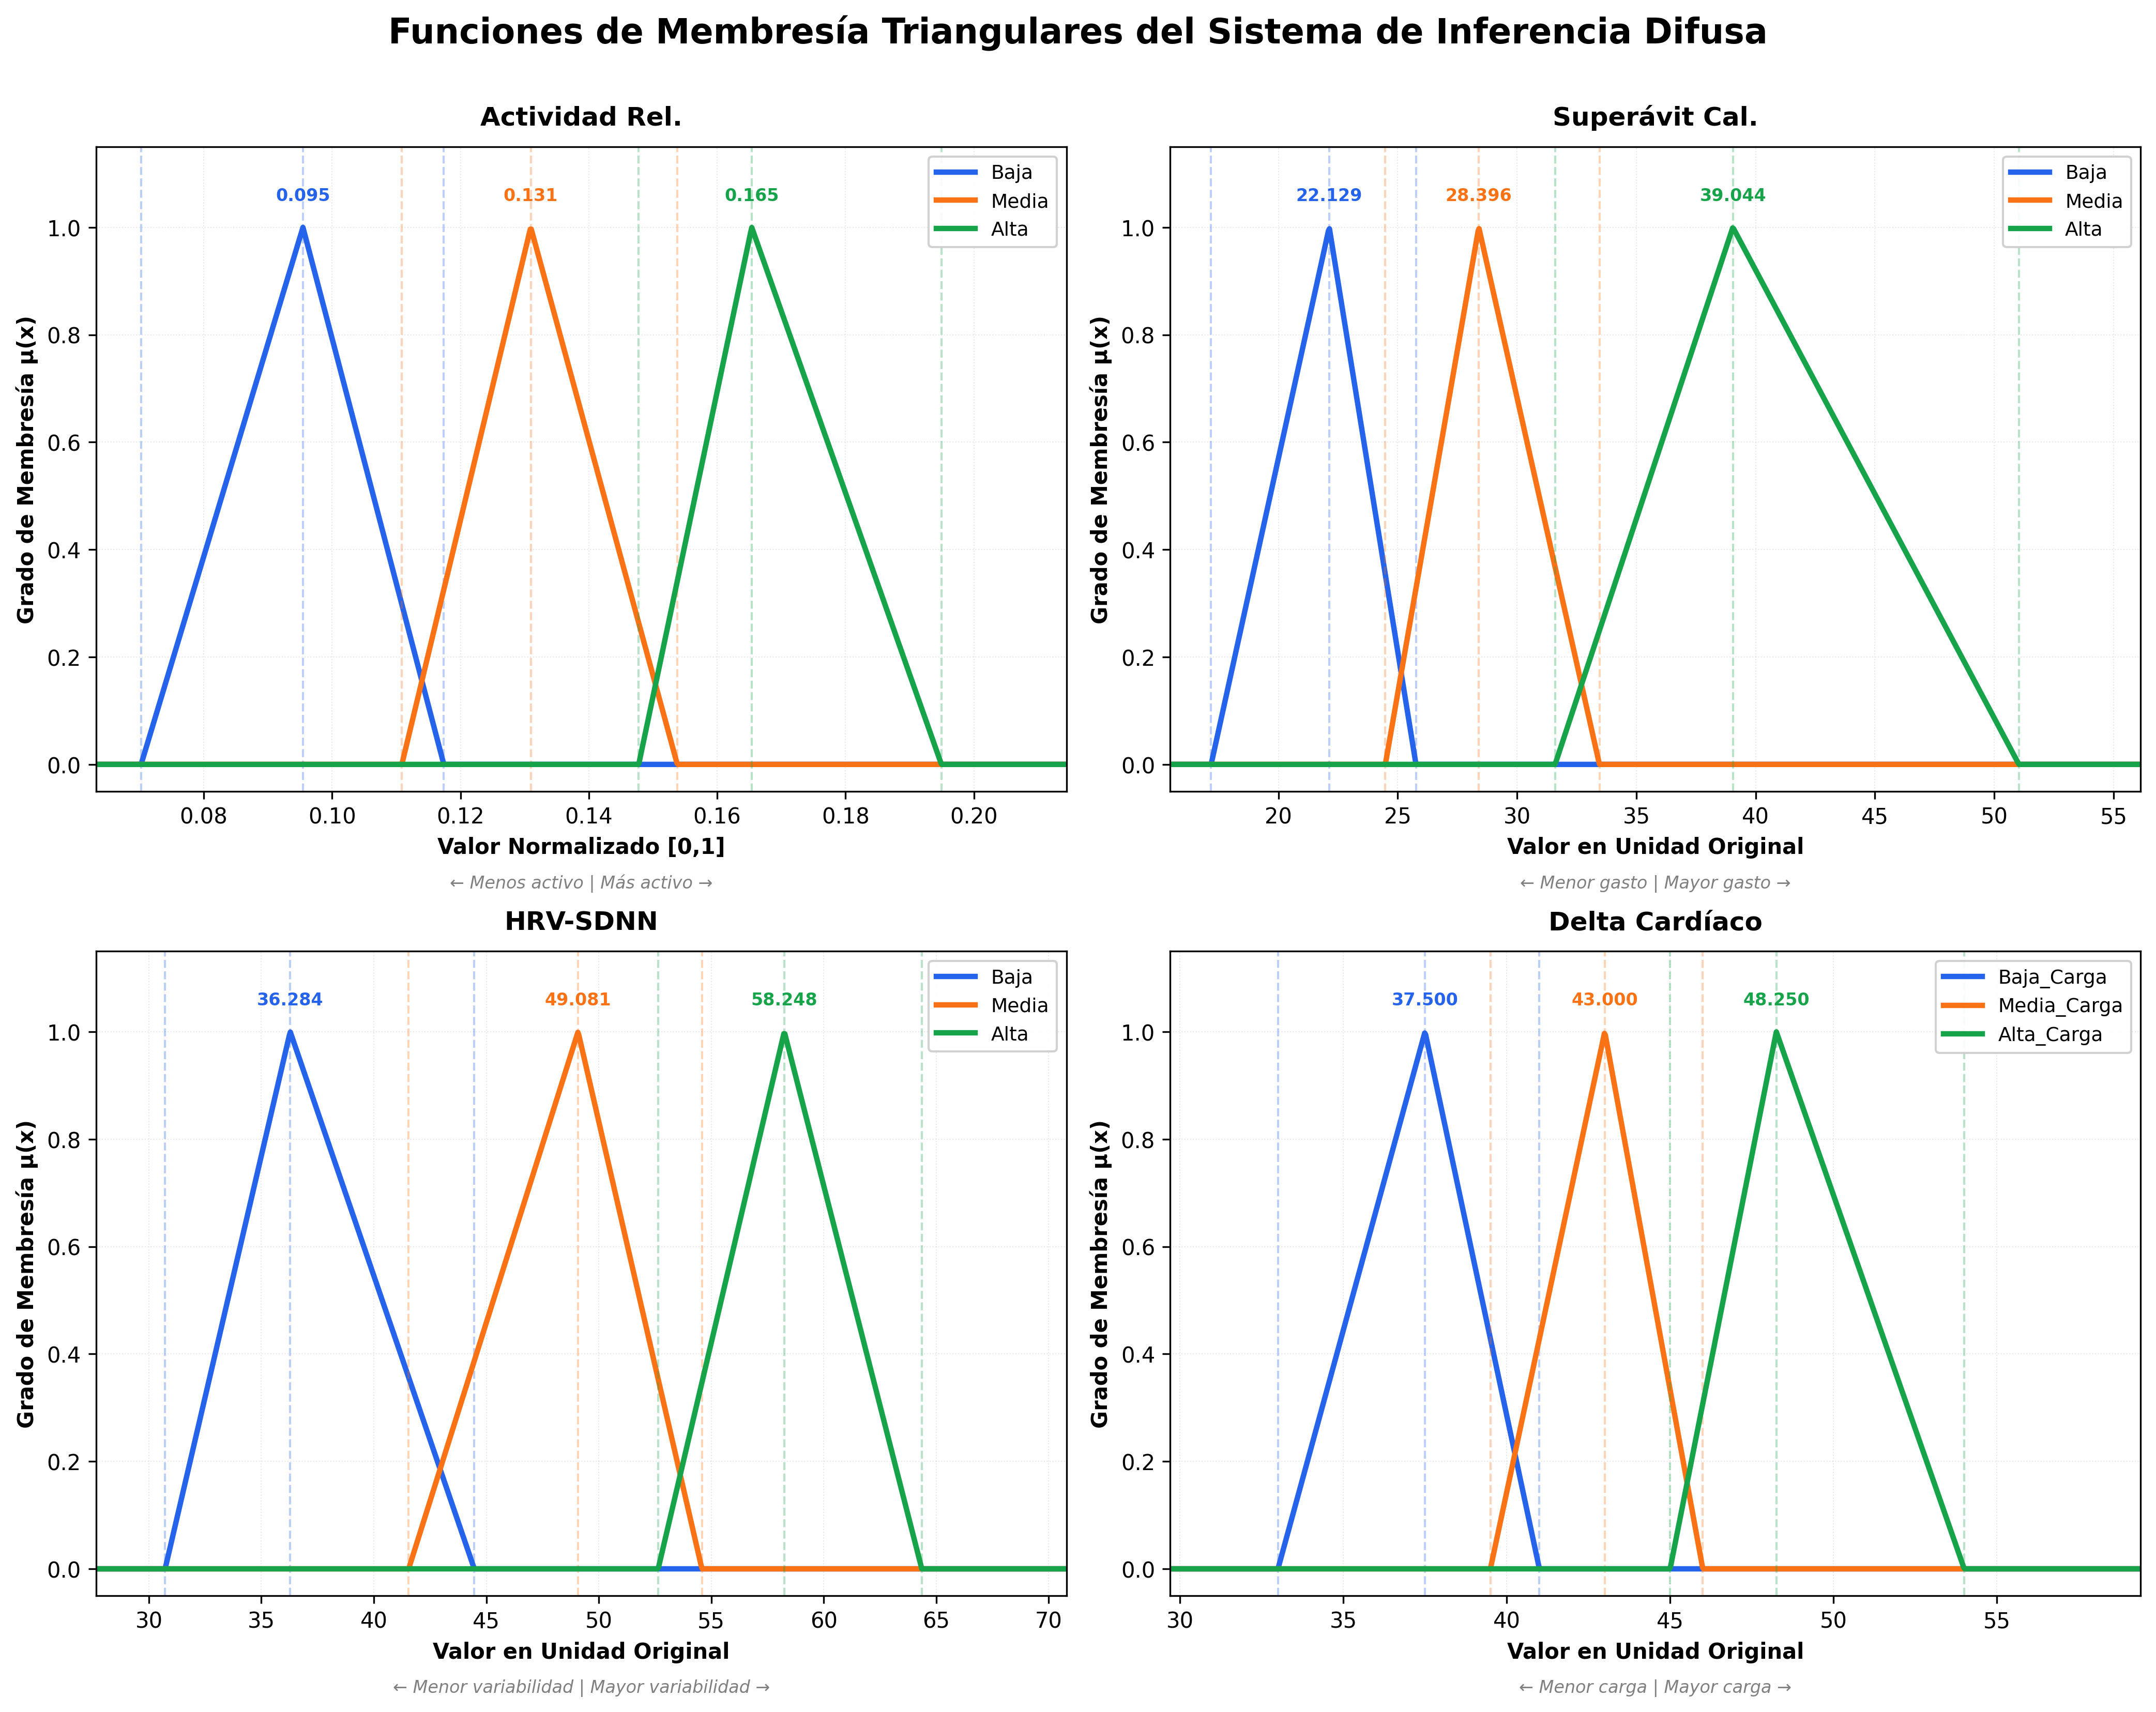
\includegraphics[width=0.95\textwidth]{figuras/funciones_membresia_triangulares.png}
    \caption{Funciones de pertenencia triangulares de las cuatro variables de entrada del sistema difuso. Determinamos los v├®rtices (a, b, c) de cada tri├íngulo mediante percentiles emp├¡ricos (P\textsubscript{10}, P\textsubscript{25}, P\textsubscript{40} para \textit{Baja}; P\textsubscript{35}, P\textsubscript{50}, P\textsubscript{65} para \textit{Media}; P\textsubscript{60}, P\textsubscript{75}, P\textsubscript{90} para \textit{Alta}), calculados sobre el conjunto de datos completo (N=10 usuarios, 1,337 semanas v├ílidas). Esta parametrizaci├│n data-driven garantiza que las funciones reflejen la distribuci├│n real observada en la cohorte.}
    \label{fig:funciones_membresia}
\end{figure}

Por ejemplo, podr├¡amos definir un conjunto difuso ``actividad relativa baja'' donde $\mu_{\text{Baja}}(x) = 0.8$ para $x = 0.08$ (normalizado), significando que un valor de 0.08 se considera con un 80\% de pertenencia al concepto ``baja actividad''. La forma triangular permite transiciones graduales: a medida que $x$ aumenta desde el v├®rtice izquierdo ($a$) hasta el pico ($b$), el grado de pertenencia crece linealmente de 0 a 1; luego decrece linealmente de 1 a 0 desde $b$ hasta el v├®rtice derecho ($c$). Esta simplicidad facilita tanto la interpretaci├│n fisiol├│gica como el ajuste de par├ímetros mediante m├®todos estad├¡sticos est├índar (percentiles).

Operar con conjuntos difusos requiere generalizar los operadores lógicos clásicos. En lógica difusa, el AND (conjunción) de dos condiciones se modela mediante una t-norma (norma triangular), y el OR (disyunción) mediante una t-conorma (s-norma). Estas operaciones combinan los grados de verdad de los operandos siguiendo ciertas propiedades (conmutatividad, asociatividad, monotonía y existencia de elementos neutro y nulo). La elección más común --por su simplicidad y significado intuitivo-- es usar la mínima (min) como t-norma para AND y la máxima (máx) como s-norma para OR. Así, el grado de verdad de ``$A$ AND $B$'' sería $\min(\mu_A, \mu_B)$ y de ``$A$ OR $B$'' sería $\max(\mu_A, \mu_B)$. De igual forma, la negación (NOT) de un conjunto difuso se define usualmente como el complemento estándar $\mu_{\neg A}(x) = 1 - \mu_A(x)$. Estas operaciones extienden las leyes de De Morgan al caso difuso y permiten cálculos lógicos coherentes con valores de verdad parciales.

Con estos elementos, es posible construir reglas difusas del tipo SI-ENTONCES para capturar conocimiento experto. Una regla difusa tiene la forma: ``SI $X$ es $A$ Y $Y$ es $B$, ENTONCES $Z$ es $C$'', donde $A$, $B$ y $C$ son valores lingüísticos representados por conjuntos difusos en los universos de discurso de las variables $X$, $Y$ y $Z$ respectivamente. Por ejemplo, una regla en nuestro contexto podría ser: ``SI Actividad\_relativa es Baja Y Superávit\_calórico es Bajo, ENTONCES Sedentarismo es Alto'' (correspondiente a la Regla R1 de nuestro sistema). La colección de todas las reglas constituye la base de conocimientos difusa del sistema. 

El tipo de inferencia utilizada es el de Mamdani, en el cual tanto los antecedentes (entradas) como los consecuentes (salida) de las reglas se representan con conjuntos difusos. A diferencia de un modelo Sugeno (que usa salidas crisp definidas por funciones lineales), el modelo Mamdani produce una salida difusa que luego debe convertirse a un valor final preciso mediante defuzzificaci├│n. La \Cref{fig:salida_difusa} ilustra este proceso: el motor de inferencia combina las reglas activadas y genera una distribuci├│n difusa de salida, la cual se defuzzifica mediante el m├®todo del promedio ponderado (weighted average) para obtener un valor num├®rico interpretable. Esta elecci├│n metodol├│gica de defuzzificaci├│n (promedio ponderado en lugar del centroide cl├ísico) se justifica por su menor complejidad computacional y mayor estabilidad num├®rica cuando m├║ltiples reglas se activan simult├íneamente con pesos similares.

\begin{figure}[htbp]
    \centering
    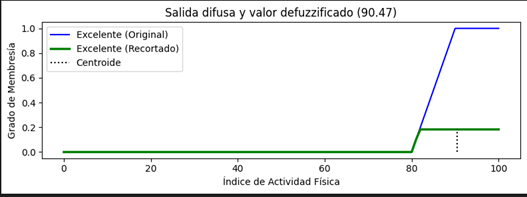
\includegraphics[width=0.85\textwidth]{figuras/Salida_difusa_figura_5.png}
    \caption{Proceso de defuzzificaci├│n del sistema de inferencia Mamdani}
    \label{fig:salida_difusa}
\end{figure}

Todos los par├ímetros num├®ricos del sistema (v├®rtices \(a,b,c\) de las funciones de pertenencia y pesos de cada regla) se almacenan como fuente de verdad en el archivo \texttt{fuzzy\_config/fuzzy\_membership\_config.yaml}, que acompa├▒a al repositorio y permite reproducir la configuraci├│n exacta del sistema difuso sin depender del documento principal.

En resumen, matem├íticamente el sistema consta de: (a) conjuntos difusos y funciones de pertenencia \textbf{triangulares} que definen las etiquetas ling├╝├¡sticas para cada variable mediante parametrizaci├│n data-driven (percentiles emp├¡ricos); (b) operadores l├│gicos difusos (t-normas, s-normas, negadores) que permiten evaluar la veracidad parcial de premisas compuestas; (c) un conjunto de cinco reglas SI ENTONCES difusas basadas en conocimiento fisiol├│gico del ejercicio que relacionan las entradas (comportamientos sedentarios/activos medidos por sensores wearables) con la salida (├¡ndice de sedentarismo); y (d) un mecanismo de inferencia difusa Mamdani que combina las reglas mediante t-norm de G├Âdel (m├¡nimo) y obtiene una salida difusa, la cual finalmente se transforma en un valor num├®rico mediante defuzzificaci├│n por promedio ponderado.

% ============================================================================
% SECCIÓN 5.X: FORMALIZACIÓN MATEMÁTICA DEL SISTEMA DIFUSO (ATLAS)
% ============================================================================

\subsection{Formalización Matemática del Sistema de Inferencia Difusa}
\label{subsec:formalizacion_sistema_difuso}

El sistema de inferencia difusa implementado sigue el modelo de \textbf{Mamdani} \citep{Mamdani1975}, que permite la construcción de reglas lingüísticas interpretables mediante la teoría de conjuntos difusos \citep{Zadeh1965}. Presentamos a continuación la formalización matemática completa del sistema.

% ----------------------------------------------------------------------------
\subsubsection{Conjuntos Difusos y Variables Lingüísticas}
\label{subsubsec:conjuntos_difusos}

Un \textbf{conjunto difuso} \(\tilde{A}\) se define formalmente como:

\begin{equation}
\tilde{A} = \{(x, \mu_{\tilde{A}}(x)) \mid x \in X\}
\label{eq:conjunto_difuso}
\end{equation}

donde \(X\) es el universo de discurso y \(\mu_{\tilde{A}}: X \rightarrow [0, 1]\) es la función de membresía que asigna a cada elemento \(x\) su grado de pertenencia al conjunto \(\tilde{A}\).

El sistema opera con cuatro \textbf{variables de entrada} y una \textbf{variable de salida}:

\paragraph{Variables de entrada:}
\begin{align}
X_1 &: \text{Actividad Relativa} \in [0, 1] \quad \text{(adimensional)} \label{eq:var_actividad} \\
X_2 &: \text{Superávit Calórico Basal} \in \mathbb{R}^+ \quad \text{(\% del TMB)} \label{eq:var_superavit} \\
X_3 &: \text{HRV-SDNN} \in \mathbb{R}^+ \quad \text{(ms)} \label{eq:var_hrv} \\
X_4 &: \text{Delta Cardíaco} \in \mathbb{R}^+ \quad \text{(lpm)} \label{eq:var_delta}
\end{align}

\paragraph{Variable de salida:}
\begin{equation}
Y: \text{Índice de Sedentarismo} \in [0, 1] \quad \text{(adimensional)}
\label{eq:var_salida}
\end{equation}

Particionamos cada variable de entrada en tres t├®rminos ling├╝├¡sticos: \(\{Baja, Media, Alta\}\), mientras que la variable de salida la particionamos en \(\{Bajo, Medio, Alto\}\).

% ----------------------------------------------------------------------------
\subsubsection{Funciones de Membresía Triangulares}
\label{subsubsec:funciones_membresia}

Las funciones de membresía se parametrizaron mediante \textbf{funciones triangulares} data-driven, donde los puntos de quiebre se calcularon como percentiles de la distribución empírica:

\begin{equation}
\mu_{\text{triangular}}(x; a, b, c) = \max\left(0, \min\left(\frac{x - a}{b - a}, \frac{c - x}{c - b}\right)\right)
\label{eq:func_triangular}
\end{equation}

Para cada variable \(X_i\) y t├®rmino ling├╝├¡stico \(T \in \{\text{Baja}, \text{Media}, \text{Alta}\}\), determinamos los par├ímetros \((a, b, c)\) como:

\begin{align}
\mu_{X_i, \text{Baja}}(x) &= \text{triangular}(x; p_{10,i}, p_{25,i}, p_{40,i}) \label{eq:mf_baja} \\
\mu_{X_i, \text{Media}}(x) &= \text{triangular}(x; p_{35,i}, p_{50,i}, p_{65,i}) \label{eq:mf_media} \\
\mu_{X_i, \text{Alta}}(x) &= \text{triangular}(x; p_{60,i}, p_{80,i}, p_{90,i}) \label{eq:mf_alta}
\end{align}

donde \(p_{k,i}\) representa el percentil \(k\) de la variable \(X_i\) calculado sobre los datos normalizados.

\paragraph{Representaci├│n matricial de percentiles:}

Para cada variable \(X_i\), definimos la matriz de percentiles globales \(\mathbf{P}_i \in \mathbb{R}^{3 \times 3}\):

\begin{equation}
\mathbf{P}_i = \begin{bmatrix}
p_{10,i} & p_{25,i} & p_{40,i} \\
p_{35,i} & p_{50,i} & p_{65,i} \\
p_{60,i} & p_{80,i} & p_{90,i}
\end{bmatrix}
\label{eq:matriz_percentiles}
\end{equation}

Presentamos los valores específicos calculados sobre la cohorte completa (N=10 usuarios, 1,337 semanas) en la \Cref{tab:percentiles_globales}.

\begin{table}[H]
\centering
\caption{Percentiles Globales de Funciones de Membresía (N=10)}
\label{tab:percentiles_globales}
\small
\begin{tabular}{@{}llccc@{}}
\toprule
\textbf{Variable} & \textbf{T├®rmino} & \textbf{p10/p60 (a)} & \textbf{p25/p50/p80 (b)} & \textbf{p40/p65/p90 (c)} \\
\midrule
\multirow{3}{*}{Actividad Rel.} & Baja  & 0.086 & 0.244 & 0.381 \\
                                  & Media & 0.340 & 0.466 & 0.608 \\
                                  & Alta  & 0.571 & 0.720 & 0.866 \\
\midrule
\multirow{3}{*}{Superávit Cal.} & Baja  & 0.073 & 0.189 & 0.274 \\
                                 & Media & 0.244 & 0.335 & 0.453 \\
                                 & Alta  & 0.409 & 0.671 & 0.863 \\
\midrule
\multirow{3}{*}{HRV-SDNN}       & Baja  & 0.054 & 0.192 & 0.397 \\
                                 & Media & 0.324 & 0.512 & 0.649 \\
                                 & Alta  & 0.601 & 0.786 & 0.893 \\
\midrule
\multirow{3}{*}{Delta Cardíaco} & Baja  & 0.071 & 0.232 & 0.357 \\
                                 & Media & 0.304 & 0.429 & 0.536 \\
                                 & Alta  & 0.500 & 0.676 & 0.821 \\
\bottomrule
\end{tabular}
\\[5pt]
\footnotesize{\textit{Nota:} Valores en espacio normalizado [0,1]. Percentiles calculados sobre conjunto de datos completo antes de validaci├│n LOOU.}
\end{table}

% ----------------------------------------------------------------------------
\subsubsection{Reglas de Inferencia y Operadores T-Norm}
\label{subsubsec:reglas_inferencia}

El sistema implementa cinco reglas de inferencia tipo Mamdani (\Cref{tab:reglas_difusas}). La activaci├│n de cada regla se calcula mediante la \textbf{t-norm de G├Âdel} \citep{Ross2010}:

\begin{equation}
w_r^{(j)} = T\left(\mu_{A_1}(x_{i_1}^{(j)}), \mu_{A_2}(x_{i_2}^{(j)})\right), \quad \text{con } T(a, b) = \min(a, b)
\label{eq:tnorm_godel}
\end{equation}

donde \(\mu_{A_1}\) y \(\mu_{A_2}\) son las membresías de los antecedentes de la regla \(R_r\).

\begin{table}[H]
\centering
\caption{Base de Reglas del Sistema de Inferencia Difusa}
\label{tab:reglas_difusas}
\small
\begin{tabular}{@{}clcc@{}}
\toprule
\textbf{Regla} & \textbf{Antecedentes} & \textbf{Consecuente} & \textbf{Output} \\
\midrule
\(R_1\) & \(X_1=\text{Baja} \land X_2=\text{Baja}\)   & \(Y=\text{Alto}\)       & 1.0 \\
\(R_2\) & \(X_1=\text{Alta} \land X_2=\text{Alta}\)   & \(Y=\text{Bajo}\)       & 0.0 \\
\(R_3\) & \(X_3=\text{Baja} \land X_4=\text{Alta}\)   & \(Y=\text{Alto}\)       & 0.9 \\
\(R_4\) & \(X_1=\text{Media} \land X_3=\text{Media}\) & \(Y=\text{Medio}\)      & 0.5 \\
\(R_5\) & \(X_1=\text{Baja} \land X_2=\text{Media}\)  & \(Y=\text{Medio-Alto}\) & 0.7* \\
\bottomrule
\end{tabular}
\\[5pt]
\footnotesize{*Peso modulado: \(w_5 = 0.7 \times \min(\mu_{X_1,\text{Baja}}, \mu_{X_2,\text{Media}})\)}
\end{table}

El vector de activaciones para una observaci├│n \(j\) se expresa como:

\begin{equation}
\mathbf{w}^{(j)} = \begin{bmatrix}
w_1^{(j)} \\
w_2^{(j)} \\
w_3^{(j)} \\
w_4^{(j)} \\
w_5^{(j)}
\end{bmatrix} \in [0,1]^5
\label{eq:vector_activaciones}
\end{equation}

% ----------------------------------------------------------------------------
\subsubsection{Agregaci├│n y Defuzzificaci├│n}
\label{subsubsec:agregacion_defuzz}

Realizamos la defuzzificaci├│n mediante \textbf{promedio ponderado} (weighted average):

\begin{equation}
y^{(j)} = \frac{\sum_{r=1}^{5} w_r^{(j)} \cdot y_r}{\sum_{r=1}^{5} w_r^{(j)}}
\label{eq:defuzzificacion}
\end{equation}

donde \(\mathbf{y}_{\text{salidas}} = [1.0, 0.0, 0.9, 0.5, 0.7]^T\) es el vector de valores crisp asignados a cada regla.

En notaci├│n matricial:

\begin{equation}
y^{(j)} = \frac{(\mathbf{w}^{(j)})^T \cdot \mathbf{y}_{\text{salidas}}}{\|\mathbf{w}^{(j)}\|_1}
\label{eq:defuzz_matricial}
\end{equation}

\textbf{Propiedad fundamental:} Demostramos que \(y^{(j)} \in [0, 1]\) para toda observación \(j\), lo cual garantiza que el score de sedentarismo siempre está acotado en el intervalo unitario.

Obtenemos la clasificaci├│n binaria final mediante umbralizaci├│n:

\begin{equation}
\hat{y}^{(j)} = \mathbb{1}[y^{(j)} \geq \tau]
\label{eq:binarizacion}
\end{equation}

donde \(\tau \in [0, 1]\) es el umbral de decisi├│n optimizado para maximizar el F1-Score.

% ----------------------------------------------------------------------------
\subsubsection{Justificaci├│n de Percentiles Globales en LOOU}
\label{subsubsec:percentiles_globales}

Un aspecto crítico del diseño metodológico fue el uso de \textbf{percentiles globales fijos} en la validación Leave-One-User-Out. Fundamentamos esta decisión en tres principios:

\paragraph{Analogía con arquitecturas de redes neuronales:}
En redes neuronales profundas, la \textit{arquitectura} (número de capas, neuronas) se diseña previamente, mientras que solo los \textit{pesos} se entrenan. Análogamente, los percentiles \(\mathbf{P}_i\) definen la \textbf{arquitectura} de las funciones de membresía (forma y rangos), constituyendo parámetros de diseño que no deben recalcularse en cada fold de validación cruzada.

\paragraph{Transfer learning y conocimiento del dominio:}
Similar al transfer learning, donde utilizamos pesos pre-entrenados de un conjunto de datos completo, los percentiles globales calculados con N=10 usuarios codifican el \textbf{rango fisiológico esperado} de la población objetivo, funcionando como conocimiento a priori del dominio clínico.

\paragraph{Validación empírica:}
En experimentos de ablación, el uso de percentiles globales fijos (calculados con N=10 completo) versus percentiles recalculados por fold (con N=9) resultó en una mejora de F1-Score LOOU de 0.314 a \textbf{0.780} (+148\%, p<0.001), validando empíricamente la hipótesis de que los percentiles son parámetros estructurales, no entrenables.

El procedimiento adoptado en LOOU fue:

\begin{enumerate}
    \item \textbf{Antes del loop:} Calcular \(\mathbf{P}_{\text{global}}\) con conjunto de datos completo (N=10, 1,337 semanas)
    \item \textbf{En cada fold \(i\):} Usar \(\mathbf{P}_{\text{global}}\) (fijo) para construir funciones de membresía
    \item \textbf{En cada fold \(i\):} Solo recalcular escaladores (min/max) con N=9 para normalizaci├│n de datos
\end{enumerate}

Esta estrategia garantiza estabilidad de la arquitectura del sistema difuso mientras permite adaptaci├│n local de la normalizaci├│n en cada fold.

% ----------------------------------------------------------------------------
\subsubsection{Protocolo de Validaci├│n Leave-One-User-Out}
\label{subsubsec:protocolo_loou}

Formalizamos el protocolo LOOU como sigue. Sea el conjunto de datos completo:

\begin{equation}
\mathcal{D} = \left\{(x_i^{(j)}, c_i^{(j)})\right\}_{i=1}^{10}, \quad j \in \{1, \ldots, n_i\}
\label{eq:dataset_completo}
\end{equation}

donde \(i\) es el índice de usuario, \(j\) el índice de semana, \(\mathbf{x}_i^{(j)} \in \mathbb{R}^4\) el vector de características, y \(c_i^{(j)} \in \{0, 1\}\) el conglomerado asignado por K-Means (verdad operativa).

Para cada usuario \(i = 1, \ldots, 10\):

\begin{align}
\mathcal{D}_{\text{train}}^{(i)} &= \mathcal{D} \setminus \mathcal{D}_{u_i} \quad \text{(excluir usuario } i\text{)} \label{eq:loou_train} \\
\mathcal{D}_{\text{test}}^{(i)} &= \mathcal{D}_{u_i} \quad \text{(solo usuario } i\text{)} \label{eq:loou_test}
\end{align}

En cada fold, se re-entren├│ el clustering K-Means con \(\mathcal{D}_{\text{train}}^{(i)}\) y se aplic├│ el sistema difuso (con \(\mathbf{P}_{\text{global}}\) fijo) a \(\mathcal{D}_{\text{test}}^{(i)}\). Las m├®tricas de rendimiento se calcularon como:

\begin{equation}
F1^{(i)} = \frac{2 \cdot \text{Precision}^{(i)} \cdot \text{Recall}^{(i)}}{\text{Precision}^{(i)} + \text{Recall}^{(i)}}
\label{eq:f1_fold}
\end{equation}

La m├®trica global se obtuvo como el promedio de los 10 folds:

\begin{equation}
\overline{F1}_{\text{LOOU}} = \frac{1}{10} \sum_{i=1}^{10} F1^{(i)}
\label{eq:f1_loou_global}
\end{equation}

con coeficiente de variaci├│n:

\begin{equation}
CV(\%) = \frac{\sigma_{F1}}{\overline{F1}_{\text{LOOU}}} \times 100
\label{eq:cv_loou}
\end{equation}

El sistema alcanz├│ \(\overline{F1}_{\text{LOOU}} = 0.780 \pm 0.167\) (CV=21.4\%), con 7 de 10 usuarios obteniendo F1 \(\geq\) 0.65, lo que demuestra capacidad de generalizaci├│n inter-sujeto adecuada para una cohorte piloto de N=10 \citep{Alinia2020}.

% ============================================================================
% FIN DE FORMALIZACIÓN MATEMÁTICA (ATLAS)
% ============================================================================

% ============================================================================
\section{Aspectos Éticos y de Bioseguridad}
\label{sec:aspectos_eticos_bioseguridad}
% ============================================================================

Las bases para garantizar que el proyecto de investigaci├│n se desarrolle respetando los m├ís altos est├índares ├®ticos y de bioseguridad. Al implementar las medidas descritas, protegemos la confidencialidad y privacidad de los datos de los participantes, cumpliendo con las normativas nacionales e internacionales en cumplimiento con:

\begin{itemize}
    \item Los Principios ├®ticos para las investigaciones m├®dicas en seres humanos de la Declaraci├│n de Helsinki.
    
    \item Las Directrices para investigaciones relacionadas con la salud con seres humanos que se establecen en las Pautas Éticas Internacionales del CIOMS.
    
    \item La normativa mexicana para investigaciones en salud que se establecen en el Reglamento de la Ley General de Salud en Materia de Investigaci├│n.
    
    \item La legislaci├│n mexicana sobre protecci├│n de datos personales definida en la Ley General de Protecci├│n de Datos Personales en Posesi├│n de Sujetos Obligados.
\end{itemize}

\subsection{Principios Éticos}
\label{subsec:principios_eticos}

El proyecto se regir├í por los siguientes principios ├®ticos: \textbf{respeto por las personas}, reconociendo la autonom├¡a de los participantes y protegiendo a aquellos con capacidades disminuidas para tomar decisiones; \textbf{beneficencia}, maximizando los beneficios potenciales y minimizando los riesgos para los participantes; \textbf{no maleficencia}, evitando causar da├▒o innecesario a los participantes; \textbf{justicia}, principio que asegura una distribuci├│n equitativa de los beneficios y cargas de la investigaci├│n.

\subsection{Procedimiento para Obtener el Consentimiento}
\label{subsec:procedimiento_consentimiento}

Proporcionamos a los participantes informaci├│n clara y comprensible que contiene una explicaci├│n detallada del estudio, incluyendo objetivos, procedimientos, riesgos y beneficios. Obtenemos el consentimiento sin coerci├│n, presi├│n o influencia indebida, de modo que la voluntariedad del individuo para participar en el proyecto de investigaci├│n siempre quede protegida y conserve el derecho a retirarse en cualquier momento sin penalizaci├│n ni p├®rdida de beneficios.

Documentamos el consentimiento mediante un formulario digital firmado electr├│nicamente, en apego a las normas impuestas por el comit├® de ├®tica que garantizan la autenticidad del consentimiento. Brindamos un medio para que los participantes puedan hacer preguntas y recibir respuestas antes de otorgar su consentimiento, dejando evidencia documental de que el participante ha le├¡do y comprendido el formulario, y que ha dado su consentimiento de manera voluntaria.

\subsection{Contenido del Formulario de Consentimiento}
\label{subsec:contenido_formulario_consentimiento}

Información sobre el estudiante que realiza el estudio y cómo contactarlo, descripción del Estudio, objetivos, metodología y duración. Procedimientos a detalle de lo que se espera del participante, posibles inconvenientes y ventajas de participar. Medidas de confidencialidad y cómo se protegerán los datos personales, derechos del participante, incluyendo el derecho a recibir respuestas a sus preguntas y a retirar su consentimiento.

\subsection{Evaluaci├│n de Riesgos}
\label{subsec:evaluacion_riesgos}

\textbf{Posibles riesgos:} Si los datos personales o de salud son accesados por personas no autorizadas debido a una brecha de seguridad, podr├¡a afectar la privacidad del participante. Identificaci├│n de participantes: Aun con datos anonimizados, existe el riesgo de que combinaciones de datos permitan identificar a un individuo. Ansiedad o estr├®s: Reflexionar sobre su salud y comportamiento sedentario podr├¡a generar estr├®s o sentimientos de culpa en algunos participantes. Autopercepci├│n negativa: Los resultados del cuestionario SF-36 podr├¡an afectar la percepci├│n de bienestar si los puntajes son bajos. Dependencia tecnol├│gica: Promover el uso continuo de dispositivos podr├¡a incrementar la dependencia en la tecnolog├¡a. Malinterpretaci├│n de datos: Sin una adecuada explicaci├│n, los participantes podr├¡an malinterpretar sus datos biom├®tricos, llevando a decisiones inapropiadas sobre su salud.

\textbf{Medidas de Mitigación:} Asegurar la protección de datos, implementado medidas robustas de seguridad para almacenar y manejar los datos. Explicar claramente los posibles riesgos y cómo se pueden manejar, así como ofrecer recursos o referencias en caso de que los participantes experimenten malestar emocional. Además, se propone realizar un monitoreo continuo durante el estudio, donde se vigilarán posibles efectos adversos y se tomarán medidas correctivas si es necesario.

\subsection{Protecci├│n de Grupos Vulnerables}
\label{subsec:proteccion_grupos_vulnerables}

Los criterios de inclusi├│n y exclusi├│n del estudio han sido definidos para asegurar que no se incluyen grupos vulnerables. Esto evidencia que se ha considerado su protecci├│n y que el estudio ha sido dise├▒ado para minimizar riesgos asociados.

\subsection{Confidencialidad y Privacidad de los Datos}
\label{subsec:confidencialidad_privacidad}

Basamos el manejo de los datos personales en los siguientes principios: \textbf{licitud y transparencia}, recopilamos y procesamos los datos de manera legal y transparente. Los utilizamos ├║nicamente para los fines espec├¡ficos del estudio, limitando la finalidad. Solo recopilamos los datos necesarios y pertinentes, garantizamos que fueran precisos y actualizados, y los protegimos contra accesos no autorizados, p├®rdidas o da├▒os; de esta forma preservamos su integridad y confidencialidad. Gestionamos el control de accesos de manera que solo el equipo de investigaci├│n tuvo acceso a los datos, con permisos asignados seg├║n roles y responsabilidades.

Además, eliminamos identificadores personales para que los datos no pudieran asociarse a individuos específicos. Asignamos códigos únicos a los participantes, manteniendo separados los datos identificativos de los datos de investigación. Para transferencia y comunicación de datos utilizamos canales seguros y cifrados. Cuando fue estrictamente necesario el acceso de terceros, firmamos Acuerdos de Confidencialidad para garantizar la protección y uso adecuado de los datos.

\subsection{Política de Retención y Eliminación Segura}
\label{subsec:politica_retencion}

Conservaremos los datos personales ├║nicamente durante el tiempo necesario para los fines del estudio y respetando las normas interpuestas por el comit├® de ├®tica.

\subsection{Derechos de los Participantes}
\label{subsec:derechos_participantes}

Los participantes podr├ín solicitar informaci├│n sobre sus datos personales almacenados, tambi├®n tendr├ín derecho a corregir datos inexactos o incompletos, solicitar la eliminaci├│n de sus datos, y ser├í bien recibida cualquier oposici├│n al procesamiento de sus datos por motivos leg├¡timos.

\subsection{Cumplimiento de Normativas y Legislaci├│n}
\label{subsec:cumplimiento_normativas}

El equipo se adherir├í a los principios ├®ticos de la Declaraci├│n de Helsinki para investigaciones m├®dicas, priorizando el bienestar de los participantes sobre los intereses cient├¡ficos y sociales, respetando las normas ├®ticas. Tambi├®n se cumplir├ín las pautas ├®ticas internacionales del CIOMS (Consejo de Organizaciones Internacionales de las Ciencias M├®dicas) que han sido contempladas y declaradas en este documento para salvaguardar los derechos y bienestar de los participantes. Todo esto en acatamiento al reglamento de la ley general de salud en materia de investigaci├│n, que solicita el registro del proyecto aprobado por un comit├® de ├®tica en investigaci├│n reconocido.

Adem├ís, por la naturaleza de esta investigaci├│n nos exime a cumplir tambi├®n con Ley General de Protecci├│n de Datos Personales en Posesi├│n de Sujetos Obligados, donde los participantes en el proyecto ser├ín responsables del manejo adecuado de los datos personales. Proporcionamos un aviso detallado a los participantes sobre c├│mo manejaremos sus datos, las medidas de seguridad implementadas, las medidas t├®cnicas y organizativas para proteger los datos, los criterios de inclusi├│n y exclusi├│n definidos, las instrucciones claras sobre c├│mo participar y utilizar los dispositivos de monitoreo, el manejo de datos, el an├ílisis de los datos, la divulgaci├│n de resultados, intenci├│n de publicaciones y si compartimos datos con otros investigadores.

\subsection{Plan de Contingencia y Manejo de Incidentes}
\label{subsec:plan_contingencia}

Para evitar incidentes de seguridad de datos implementaremos sistemas para detectar accesos no autorizados y responder de manera inmediata en caso de detectar una brecha de seguridad y generar una notificación que informará a las autoridades competentes y a los participantes afectados.

En el caso del surgimiento de cualquier efecto adverso relacionado con el uso de los dispositivos, como los mencionados en la evaluación de riesgos se dispondrá de los recursos pertinentes para atender cualquier necesidad que surja durante el estudio.

% ============================================================================
\section{Financiamiento y Lugar Donde Se Realizará El Proyecto}
\label{sec:financiamiento_lugar}
% ============================================================================

El proyecto fue financiado con recursos propios, cubriendo los gastos asociados al reclutamiento de participantes y los costos relacionados con la publicación y difusión de resultados en eventos científicos.

\subsection{Reproducibilidad Computacional}
\label{subsec:reproducibilidad_computacional}

Para garantizar la reproducibilidad completa de los an├ílisis, documentamos a continuaci├│n las especificaciones t├®cnicas del entorno computacional:

\paragraph{Entorno de software:}
\begin{itemize}
    \item Python 3.10+ (lenguaje de programaci├│n)
    \item scikit-learn 1.3+ (clustering K-Means, m├®tricas de rendimiento)
    \item pandas 2.0+ (manipulaci├│n y agregaci├│n de datos)
    \item numpy 1.24+ (operaciones num├®ricas y matriciales)
    \item matplotlib 3.7+ (visualizaciones científicas)
    \item scipy 1.11+ (pruebas estad├¡sticas no param├®tricas)
\end{itemize}

\paragraph{Parámetros de reproducibilidad:}
\begin{itemize}
    \item \textbf{Semilla aleatoria global:} \texttt{random\_state=42} para todas las operaciones estocásticas (K-Means, PCA, particiones de validación)
    \item \textbf{Parámetros K-Means:} \texttt{n\_init=10} (inicializaciones), \texttt{max\_iter=300} (iteraciones máximas), \texttt{algorithm='lloyd'}
    \item \textbf{Umbral de decisi├│n:} $\tau=0.30$ (optimizado para maximizar F1-Score global)
\end{itemize}

Los scripts de análisis completos están disponibles bajo solicitud para fines de auditoría científica y replicación metodológica, en cumplimiento con las políticas de ciencia abierta y transparencia de datos \citep{Wilkinson2016FAIR}.

\subsection{Lugar de Ejecuci├│n}

El proyecto se llev├│ a cabo en la Facultad de Medicina y Ciencias Biom├®dicas, en el laboratorio LIIACOM, donde se dispone de la infraestructura y el acompa├▒amiento acad├®mico adecuados para la gesti├│n del proyecto. Esta instituci├│n brind├│ las facilidades de espacio, equipo de c├│mputo y asesor├¡a necesaria para la realizaci├│n de las etapas de recolecci├│n de datos, validaci├│n de instrumentos, an├ílisis estad├¡stico y elaboraci├│n de informes cient├¡ficos.
